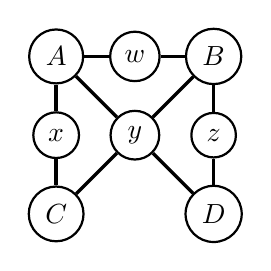
\begin{tikzpicture}
\begin{scope}[every node/.style={circle,thick,draw}]
    \node (C) at (-1,-1) {$C$};
    \node (x) at (-1,0) {$x$};
    \node (A) at (-1,1) {$A$};
    \node (y) at (0,0) {$y$};
    \node (w) at (0,1) {$w$};
    \node (D) at (1,-1) {$D$};
    \node (z) at (1,0) {$z$};
    \node (B) at (1,1) {$B$};
\end{scope}

\begin{scope}[every node/.style={fill=white,circle},
              every edge/.style={draw=black,very thick}]
    \path [-] (A) edge (w);
    \path [-] (A) edge (x);
    \path [-] (A) edge (y);
    \path [-] (B) edge (w);
    \path [-] (B) edge (y);
    \path [-] (B) edge (z);
    \path [-] (C) edge (x);
    \path [-] (C) edge (y);
    \path [-] (D) edge (y);
    \path [-] (D) edge (z);
\end{scope}
\end{tikzpicture}